\section{Построение решений задач}
\label{sec:Chapter3} \index{Chapter3}

После анализа литературы и уже существующих решений стало ясно, как реализовывать каждую из поставленных ранее задач. Далее будет рассказано о том, какие методы были выбраны для выполнения этих задач. Порядок, в котором они были объявлены в разделе \ref{sec:Chapter1} сохранен.

\subsection{Признаки для датасета}
\label{sec:dataset} \index{dataset}

Обсудим признаки, которые были выбраны для обучения классификатора. В предыдущем разделе \ref{sec:Chapter2} было сказано, что из всех признаков, указанных в \cite{HECKMAN2011363}, данная работа сфокусируется лишь на первых двух - характеристики ошибки и характеристики кода, опуская последние три - метрики репозитория с исходным кодом, метрики базы данных с багами, метрики динамического анализа. Далее будет описано, почему при составлении датасета был опущен каждый из перечисленных классов признаков, а также будет описано то, какие признаки все же были представлены в датасете в настоящей работе.

\subsubsection{Метрики репозитория с исходным кодом}
Как было обозначено в обзоре литературы \ref{sec:Chapter2}, для того, чтобы хоть сколько нибудь эффективно анализировать историю коммитов проекта, она должна быть строго организована, иначе поиск нужных мест в коде сводится к полному анализу всего проекта на каждом из этапов его разработки. В том же разделе было объяснено, что в открытом доступе очень малое число проектов соблюдает подобные правила. Плюс, даже при их соблюдении, множественный анализ проекта очень дорог вычислительно и по времени. Плюс, для того, чтобы размечать false positives, необходимо иметь доступ к уже собранной статистике использования анализатора, которой не существует в открытом доступе. Таким образом, анализ истории коммитов и других метрик репозитория отпадает.

\subsubsection{Метрики базы данных с уязвимостями}
Как и в предыдущем пункте, применение данных метрик ограничивается их отсутствием в открытом доступе.

\subsubsection{Метрики динамического анализа}
Для проведения динамического анализа требуется полная сборка всего проекта, что добавляет сложности к и без того затратному процессу анализа. Также, основным предметом изучения данной работы является именно статический анализ, поэтому рассмотрение метрик динамического анализа было решено оставить как предмет для будущих исследований.

\subsubsection{Характеристики ошибки}
\label{sec:Err-to-CWE} \index{Err-to-CWE}
Для того, чтобы удовлетворить требованию языковой независимости, все сообщения анализаторов требуется приводить к общему виду. Таким общим видом было выбрано представление Common Weakness Enumeration (CWE)\cite{CWE-doc}. Таким образом, добавление нового статического анализатора к списку поддерживаемых сводится к добавлению интерфейса, транслирующего код ошибки анализатора в код CWE. К счастью, для большинства распространенных статических анализаторов существуют таблицы соответствия или настройки, позволяющие выводить код ошибки сразу в формате CWE.

\subsubsection{Характеристики кода}
В проанализированной литературе основными признаками, по которым производилось обучение, являлись метрики кода. Чаще всего речь шла о метриках таких как вложенность, цикломатическая сложность, количество путей через выделенный фрагмент кода, etc. В данной работе метрики кода считались только для функции, в которой анализатор обнаружил уязвимость. Замеры производились при помощи утилиты ccsm\cite{CCSM}, в которую были дополнительно внесены изменения. Реализована данная утилита как инструмент в инфраструктуре Clang\cite{Clang}. Этот инструмент вызывает парсер Clang для указанного файла, и работает с полученным частичным промежуточным представлением. Т.к. полная компиляция проекта не требуется (парсинг производится лишь на выбранном файле), то извлечение этих метрик не сказывается на общем времени сбора датасета. Метрики кода, использованные для обучения моделей в данной работе можно разделить на следующие группы:

\begin{enumerate}
    \item Количество ключевых слов, контролирующих поток исполнения программы (for, if, else, etc.)
    \item Различные способы подсчета цикломатической сложности
    \item Количество различных обращений к памяти (разименование указателя, обращение к полю, обращение к полю по указателю, etc.)
    \item Характеристики самой функции (количество путей через нее, вложенность)
\end{enumerate}

\subsubsection{Token-based представление кода}
\label{Tokens} \index{Tokens}
Описанные выше метрики характеризуют код лишь косвенно, не давая представления о его структуре. Таким образом теряется способность классификатора распознавать шаблоны, которые приводят к false positive. Чтобы бороться с этой проблемой был предложен подход на основе токенов. Токены были выбраны, т.к. анализ AST является затруднительным и более затратным. Токены, с другой стороны, можно получить еще на этапе лексического анализа. Вывод токенов был также реализован в качестве инструмента для Clang. Чтобы увеличить шансы на распознавание шаблонов false positive, представление кода в виде токенов было предварительно обработано: были оставлены только ключевые слова, влияющие на поток исполнения, операторы и идентификаторы.

\begin{figure}[H]
    \centering
    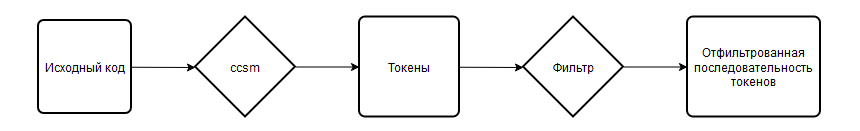
\includegraphics[width=\textwidth]{flow.png}
    \caption{Шаги получения отфильтрованной последовательности токенов}
\end{figure}

После предварительной обработки, из получившейся последовательности токенов выбирается подпоследовательность фиксированной длины, такая, что токен, на который указывает сообщение об ошибке находится ровно посередине подпоследовательности. Получившаяся подпоследовательность фиксированной длины называется окном и контролируется гиперпараметром WINDOW\_SIZE, отвечающим за ширину этого окна. Соответственно, в датасете появляются признаки token[0], token[1], token[2], ... token[WINDOW\_SIZE - 1]. Предположение данной работы состоит в том, что последовательности отфильтрованных токенов наряду с метаданными о коде должно хватить для распознавания большинства шаблонов false positive, указанных в \cite{Reynolds}.
\\
\\
Резюмируя, датасет, используемый для обучения моделей в данной работе, имеет следующий вид:

\begin{table}[H]
    \centering
    \resizebox{\textwidth}{!}{
        \begin{tabular}{|c|c|c|c|c|c||c|}
            \hline
            код CWE & token[0] & token[1] & ... & token[WINDOW\_SIZE - 1] & метрики кода & метка класса \\ \hline
        \end{tabular}
    }
    \caption{Общий вид элемента датасета}
\end{table}

\subsection{Метод генерации и разметки датасета}
Для генерации и разметки датасета была выбрана кодовая база Juliet Test Suite\cite{Juliet}. Имеющиеся в коде метаданные позволяют без проблем классифицировать большинство сообщений анализатора как false positive или true positive. Рассмотрим пример кода Juliet Test Suite:

\begin{verbatim}
    // CWE415_Double_Free__malloc_free_char_08.c
    ...
    void CWE415_Double_Free__malloc_free_char_08_bad()
    {
        ...
    }
    ...

    // manifest.xml
    ...
    <testcase>
      <file path="CWE415_Double_Free__malloc_free_char_08.c">
        <flaw line="47" name="CWE-415: Double Free"/>
      </file>
    </testcase>
    ...
\end{verbatim}

Juliet Test Suite содержит два типа метаданных, которые полезны при оценке верности предупреждений анализатора:
\begin{enumerate}
    \item manifest.xml - этот файл содержит точную информацию о каждой ошибке, включая номер строки, файл и тип ошибки.
    \item Названия функций - в документации к тестовой сюите говорится, что если название функции содержит строку 'GOOD', то указанный тип CWE в данной функции не встречается, а если название функции содержит строку 'BAD', то данный CWE в этой функции присутствует.
\end{enumerate}

Для разметки датасета были собраны следующие данные: для каждого файла, в котором анализаторы находили уязвимости были собраны метрики кода, а также token-based представление для каждой из функций. Далее стоит учитывать, что Juliet Test Suite указывает только на наличие или отсутствие конкретного CWE, указанного в названии файла, тоесть мы не можем выносить суждение о других типах уязвимостей, о которых сообщил анализатор в данном файле. Иными словами, если уязвимость, найденная анализатором не совпадает с CWE, указанным в manifest.xml или названии файла, то метаданные не могут быть использованы для того, чтобы пометить данное сообщение анализатора как true positive / false positive. Таким образом, после того, как вся тестовая сюита была проанализирована несколькими анализаторами, их сообщения об уязвимостях были слиты в единую базу данных, где каждый код ошибки был предварительно заменен на эквивалентный CWE либо при помощи встроенных в анализатор средств, либо при помощи уже заранее составленных таблиц соответствия. Далее, для каждого сообщения об ошибке была получена метка класса. Разметка происходила следующим образом:

\begin{enumerate}
    \item Если информация об уязвимости в manifest.xml (путь, строка, тип) совпадает с той, которую сообщил анализатор, то ставилась метка true positive
    \item Если уязвимость обнаружена в строках, принадлежащих функции с именем 'GOOD', и код ошибки совпадает с CWE, указанным в имени файла, то ставилась метка false positive.
\end{enumerate}

Для остальных случаев невозможно точно определить метку. Однако существуют спекулятивные методы, которые являются предметом для дальнейших исследований и не были рассмотрены в данной работе. Их применение позволит расширить кодовую базу, на которой обучается классификатор, что увеличит качество и количество распознаваемых шаблонов false positive.

\subsection{Обучение классификатора}

Выше было введено понятие обучения классификатора на размеченном датасете. Далее будут пояснены все использованные выше термины, такие как датасет, а также будут объяснены детали каждой из используемых моделей.

\subsection{Обучение с учителем}

Задачей машинного обучения является поиск функции, максимально приближающей заданную зависимость между элементами множества $X$ (объектами) и элементами множества $Y$ (таргетами), т.е. поиск $f(X):$
\[f(X) = Y + \varepsilon\]
где $\varepsilon$ - случайная величина, ошибка предсказания

Функция $f(X)$, отображающая объекты в таргеты, именуется моделью, а имеющийся у нас набор объектов иногда ещё называют обучающей выборкой или датасетом. Датасет состоит из:

\begin{enumerate}
    \item Объекты (признаки) - элементы множества X
    \item Метки (таргеты) - правильные ответы для $f(X)$.
\end{enumerate}

В обучении с учителем мы хотим при помощи обучающей выборки построить модель, предсказания которой достаточно хороши. Обычно, качество предсказаний измеряют с помощью метрик качества, то есть функций, которые показывают, насколько сильно полученные предсказания, выдаваемые моделью, похожи на правильные ответы. Цель обучения обычно состоит в том, чтобы получить как можно лучшее (наибольшее или наименьшее возможное, в зависимости от ситуации) значение метрики.

Выделяют два основных типа задач обучения с учителем в зависимости от того, каким может быть множество $Y$ всех возможных ответов (таргетов):

\begin{enumerate}
    \item Регрессия - $Y \in \mathbb{R}$ или $Y \in \mathbb{R}^M$. Примерами задач регрессии является предсказание спроса на конкретный товар в конкретный день или погода на завтра (температура, влажность, давление).
    \item Классификация - $Y = \{1,...,K\}$. Предсказание принадлежности объекта к одному из $K$ классов. Например, определение предметной области для научной статьи (математика, биология, психология и т. д.). В случае $K = 2$ данная задача называется бинарная классификация. Именно эта задача и решается в данной работе. Необходимо определить, является ли объект (уязвимость, предсказанная анализатором и ее описание, как описано выше в \ref{sec:dataset}) элементом класса false positive или true positive.
\end{enumerate}

\subsubsection{Решающее дерево. Decision tree}
Одной из самых простых, но при этом эффективных для хорошо отделимых классов, моделей для решения задачи бинарной классификации является решающее дерево. Это такое бинарное дерево, в котором:
\begin{enumerate}
    \item Каждой внутренней вершине $v$ приписан предикат $B_v: X \rightarrow {0, 1}$.
    \item каждой листовой вершине $v$ приписан прогноз $c_v \in Y$, где $Y$ — область значений целевой переменной (в случае классификации листу может быть также приписан вектор вероятностей классов).
\end{enumerate}

В ходе предсказания осуществляется проход по этому дереву к некоторому листу. Для каждого объекта выборки x движение начинается из корня. В очередной внутренней вершине $v$ проход продолжится вправо, если $B_v(x)=1$, и влево, если $B_v(x)=0$. Проход продолжается до момента, пока не будет достигнут некоторый лист, и ответом алгоритма на объекте $x$ считается прогноз $c_v$, приписанный этому листу\cite{SHAD-trees}.

Предикат $B_v$ может иметь, вообще говоря, произвольную структуру, но, как правило, на практике используют просто сравнение с порогом $t \in \mathbb{R}$ по какому-то $j$-му признаку:

\[ B_v(x,j,t)=[x_j \leq t] \]

При проходе через узел дерева с данным предикатом объекты будут отправлены в правое поддерево, если значение $j$-го признака у них меньше либо равно $t$, и в левое, если больше. В дальнейшем рассказе мы будем по умолчанию использовать именно такие предикаты.

Из структуры дерева решений следует несколько интересных свойств:\cite{SHAD-trees}

\begin{enumerate}
    \item Выученная функция является кусочно-постоянной, из-за чего производная равна нулю везде, где задана. Следовательно, о градиентных методах при поиске оптимального решения можно забыть.
    \item Решающее дерево (в отличие от, например, линейной модели) не сможет экстраполировать зависимости за границы области значений обучающей выборки.
    \item Решающее дерево способно идеально приблизить обучающую выборку и ничего не выучить (тоесть такой классификатор будет обладать низкой обобщающей способностью): для этого достаточно построить такое дерево, в каждый лист которого будет попадать только один объект. Следовательно, при обучении нам надо не просто приближать обучающую выборку как можно лучше, но и стремиться оставлять дерево как можно более простым, чтобы результат обладал хорошей обобщающей способностью.
\end{enumerate}

Теперь разберемся с тем, как построить дерево. Другими словами, обучить модель. Построение дерева будем рассматривать итеративно. Пусть $X$ - исходное множество объектов обучающей выборки, а $X_m$ - множество объектов, попавших в текущий лист (в самом начале $X_m = X$). Тогда алгоритм можно описать следующим образом:

\begin{enumerate}
    \item Рассмотрим вершину $v$. Если выполнен критерий остановки (например глубина дерева или степень ветвления), то останавливаемся, объявляем эту вершину листом и ставим ей в соответствие ответ.
    \item Иначе, находим предикат $B_{j,t}$, который даст наилучшее разбиение текущего множества $X_m$ на два подмножества $X_l$ и $X_r$, максимизируя критерий ветвления $Branch(X_m,j,t)$.
    \item Рекурсивно повторяем эту процедуру для каждого образованного подмножества. При этом в каждой вершине проверяем условие остановки. Если условие выполняется, то прекращаем рекурсию и объявляем текущую вершину листом. Иначе, продолжаем рекурсивно спускаться.
\end{enumerate}

Остановимся более подробно на функции $Branch(X_m, j, t)$, т.к. ее выбор определит то, какую информацию можно будет извлечь из конечного предсказания. Для начала определим общую идею критерия ветвления. Пусть $c \in \mathbb{R}$ - ответ классификатора, тоесть метка класса, и пусть задана функция потерь $L(y_i, c)$, характеризующая то, насколько предсказание $y_i$ отличается от ответа $c$. В момент, когда мы ищем оптимальное разделение $X_m$ на $X_l$ и $X_r$, мы можем вычислить для объектов из $X_m$ то предсказание $c$, которое дало бы дерево, если бы текущая вершина была терминальной. Это предсказание $c$ должно минимизировать среднее значение функции потерь:

\[ \dfrac{1}{|X_m|} \displaystyle\sum_{(x_i,y_i) \in X_m} L(y_i, c) \]

Оптимальное значение этой величины

\[ H(X_m) = \min_{c \in Y} \dfrac{1}{|X_m|} \displaystyle\sum_{(x_i,y_i) \in X_m} L(y_i, c) \]

Называется информативностью. Чем она ниже, тем лучше объекты в листе приближаются константным значением. Определим функцию потерь решающего пня (одного узла решающего дерева):

\[ \dfrac{1}{|X_m|} \lparen \displaystyle\sum_{(x_i,y_i) \in X_l} L(y_i, c_l) +  \displaystyle\sum_{(x_i,y_i) \in X_r} L(y_i, c_r) \rparen \]

В качестве информативности удобно взять энтропию распределения классов. Пусть мы предсказываем вероятностное распределение классов $(c_1, c_2, ..., c_K)$ и пусть $p_i$ - вероятность того, что объект принадлежит классу $c_i$. Тогда для информативности имеем\cite{SHAD-trees}:

\[ H(X_m) = - \displaystyle\sum_{(x_i,y_i) \in X_m} p_k \log{p_k} \]

В случае бинарного распределения:

\[ H(X_m) = - p \log{p} - (1 - p) \log{(1 - p)} \]

Так как $p_k \in [0,1]$, то энтропия неотрицательна. Если случайная величина принимает только одно значение, то она абсолютно предсказуема и её энтропия равна 0. Наибольшего значения энтропия достигает для равномерно распределённой случайной величины - и это отражает тот факт, что среди всех величин с данной областью значений она наиболее "непредсказуема".

Однако у решающего дерева есть минусы. Самый главный - невозможность построения оптимального решения. Ниже приведен пример для решения задачи XOR. Какой бы критерий ни оптимизировали, решение никогда не приблизится к оптимальному. Картинка ниже иллюстрирует данную проблему:

\begin{figure}[H]
    \centering
    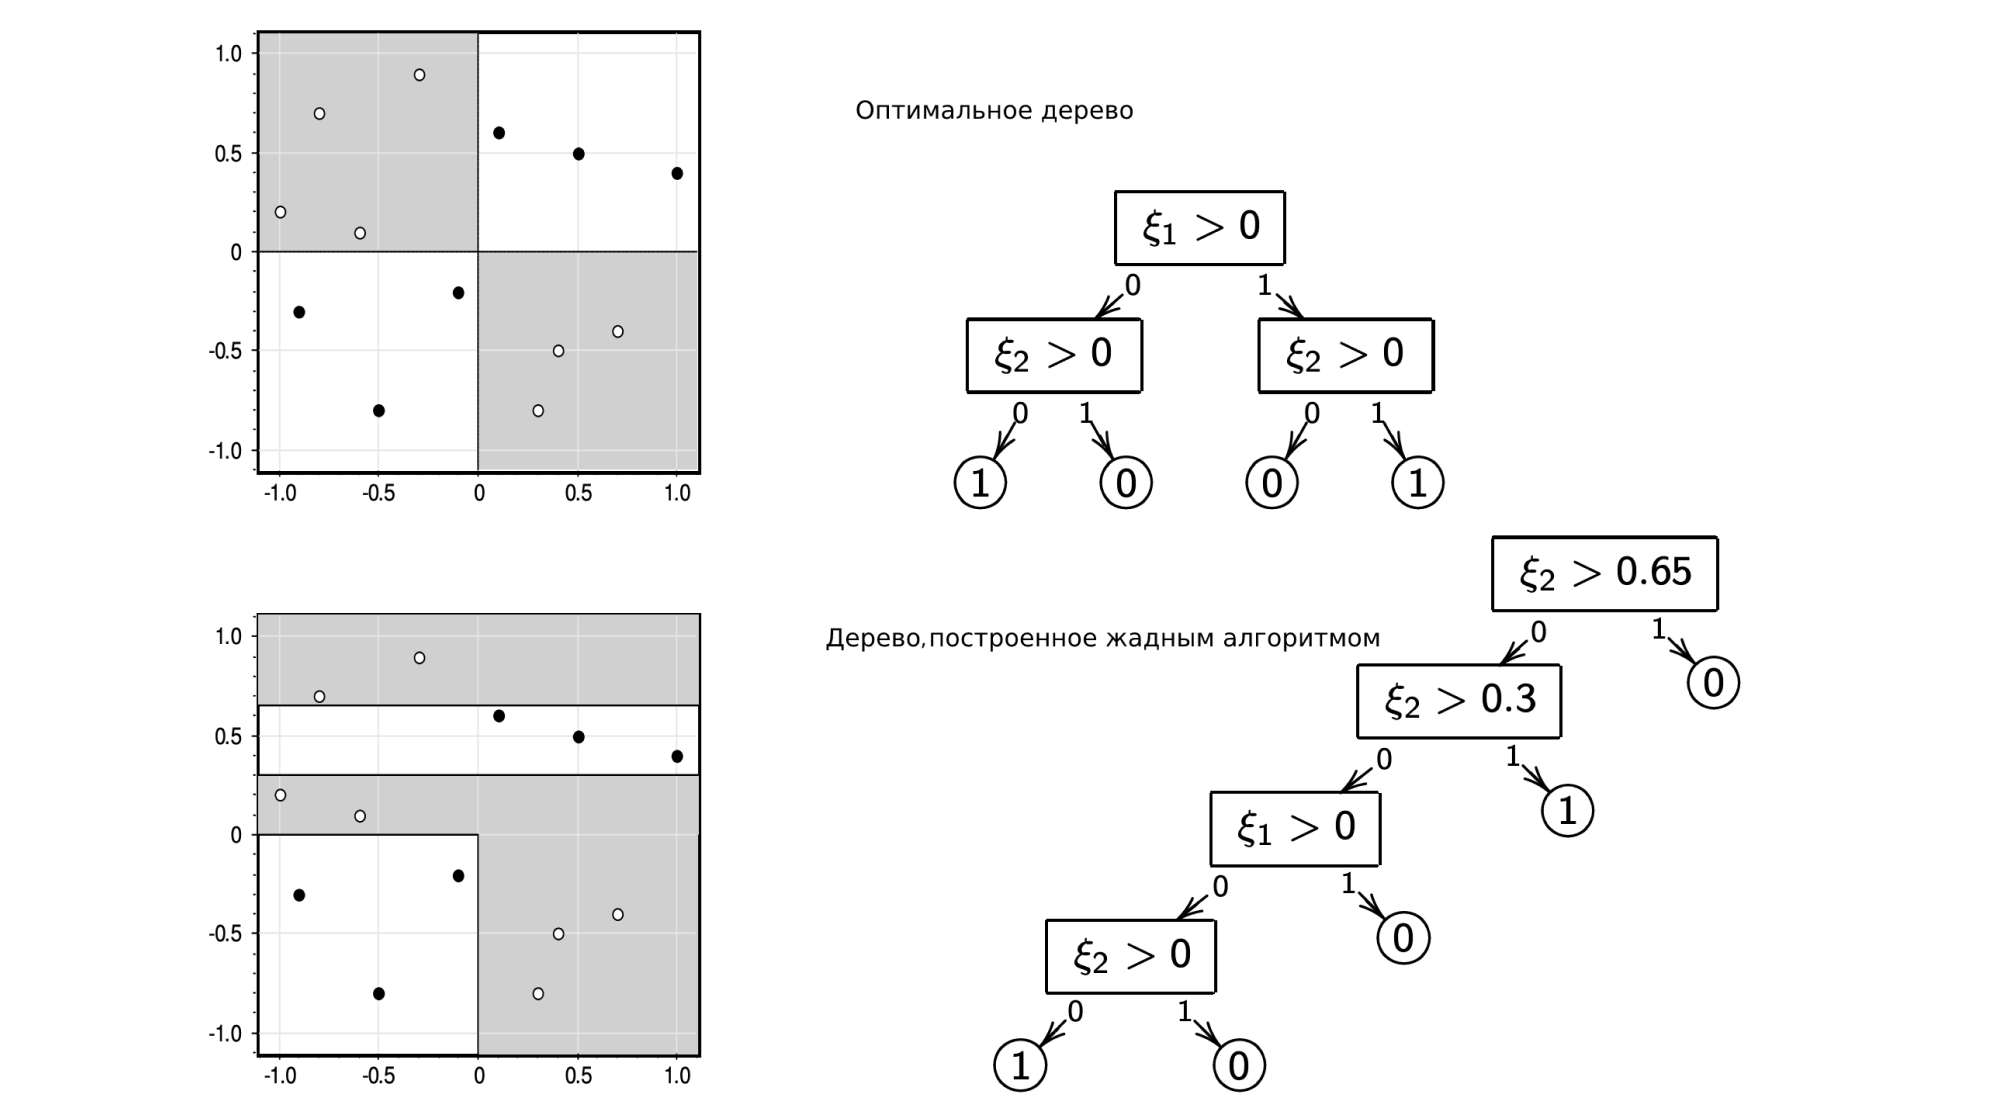
\includegraphics[width=\textwidth]{des-tree.png}
    \caption{Иллюстрация неоптимальности разбиения решающего дерева \cite{SHAD-trees}}
\end{figure}

Для того, чтобы избежать переобучения дерева (ситуации, когда обобщающая способность классификатора начинает падать из-за слишком хорошей точности на обучающей выборке), в данной работе ограничивалась глубина дерева.

\subsubsection{Градиентный бустниг. Gradient boosting}
Кратко опишем идею, стоящую за градиентным бустингом (В данной работе говорится именно о GBDT, т.е. градиентном бустинге, построенном на решающих деревьях). Эта модель хорошо показывает себя на неоднородных данных, т.е. данных, представимых в виде набора признаков, таблицы и способен хорошо находить и приближать нелинейные зависимости. Идея градиентного бустинга проста: будем использовать ансамбль простых моделей, каждая из которых плохо приближает истинную зависимость, чтобы давать предсказания. Причем каждая последующая модель в ансамбле добавляется так, чтобы уменьшить ошибку уже имеющегося ансамбля. Теперь более формально. Для решения будем строить композицию из $K$ базовых алгоритмов (в нашем случае - деревьев):

\[ a(x)= a_K(x) = b_1(x) + b_2(x) + ... + b_K(x) \]

При дальнейшем построении используется следующая идея: при обучении одного дерева $b_1(x)$ нам известны объекты, на которых его предсказание было неверным. Тогда мы можем обучить следующее дерево $b_2(x)$ предсказывать разницу $s_i^1 = y_i - b_1(x_i) = y_i - a_1(x_i)$ между результатами первого дерева и истинной зависимостью для каждого объекта обучающей выборки. Данная разница выражается через градиент функции потерь:
\[ s_i^k = y_i - a_1(x_i) = -\dfrac{\partial L(y_i, z)}{\partial z} |_{z = a_1(x_i)} \]

Или, в общем случае:

\[ s_i^k = y_i - a_k(x_i) = -\dfrac{\partial L(y_i, z)}{\partial z} |_{z = a_k(x_i)} \]
Поэтому бустинг и называется градиентным. Аналогично будет обучено третье дерево и т.д. На каждом $k$-м шаге вычисляется разница между целевой переменной и предсказанием композиции $k - 1$ алгоритмов, после чего $k$-е дерево учится предсказывать эту разницу, после чего композиция $a(x)$ обновляется:

\[ a_k(x) = a_{k-1}(x) + b_k(x) \]

Обучение K базовых алгоритмов завершает построение композиции и обучение модели.


\newpage